% !TeX spellcheck = de_DE
\documentclass[ngerman]{scrartcl} 
%\KOMAoptions{fontsize=12pt, paper=a4}
%\KOMAoptions{DIV=11}
\usepackage[ngerman]{babel}
\def\nummer{1}
\author{Cornelius Heiming}
%TODO: Name, Nummer, Datum	
\title{Versuch \nummer~:  Ausbreitung von Signalen auf Leitungen}
\date{29.04.2025}		
\usepackage{amsmath, amssymb, amsthm} 
\usepackage{geometry}
\usepackage[utf8]{inputenc}
\usepackage{enumerate}
\usepackage[shortlabels]{enumitem}

\usepackage{../pakete}
\usepackage{../aufgaben}

\addbibresource{../referenzen.bib}
\geometry{a4paper, left=3cm, right=3cm, top=3cm, bottom=3cm}

\newtheorem{theorem}{Satz}
\newtheorem{lemma}[theorem]{Lemma}
\newtheorem{korollar}{Korollar}[section]
\theoremstyle{definition}
\newtheorem{definition}[theorem]{Definition}
\newtheorem{beispiel}[theorem]{Beispiel}
\newtheorem{satz}[theorem]{Satz}

%\displaystyle \lim_{x \to \infty}

\begin{document}
	\maketitle
	\section{Einleitung}
		In diesem Versuch wird untersucht, wie Signale durch Leitungen verzögert, gedämpft und reflektiert werden. Dazu werden ein Signalgenerator, ein Oszilloskop, verschiedene Verzögerungskabel und ein Differenzierglied verwendet. Letzteres wird zunächst untersucht, um dann in der Folge als Impulsgenerator zu dienen. Diese werden dann mittels des Oszillographen in verschiedenen Konfigurationen gemessen. Danach wird der Abschluss eines Leiters und dessen Signalverzögerung untersucht. Zuletzt werden Klippkabel verwendet, um Impulse auf eine definierte Länge zu kürzen.
		%TODO Was wird gemessen?
		%TODO Wodurch ist der Versuch motiviert, was ist das Ziel des Versuches
	\section{Theorie}
		
		%TODO Kurze Darstellung der Physik für den Versuch, Grundlagen, Voraussetzungen
		%TODO Formeln, die in der Auswertung verwendet werden
		%TODO Prägnanz
		Koaxialkabel sind Leitungen, die aus einem Innenleiter und einem Außenleiter bestehen. Diese können als Kondensator aufgefasst werden, dem Kabel kann also eine Kapazität $C'$ pro Längeneinheit zugeordnet werden. Weiterhin besitzt das Kabel eine Induktivität $L'$ pro Längeneinheit. Diese beiden Größen sind gegeben durch:
		\begin{align*}
			C' &= \epsilon_r \epsilon_0\frac{2 \pi}{\ln({R_\mathrm{a}/R_\mathrm{i}})}\\
			L' &= \mu_r \mu_0\frac{\ln({R_\mathrm{a}/R_\mathrm{i}})}{2 \pi}
		\end{align*}
		mit $R_\mathrm{a}$ und $R_\mathrm{i}$ dem Außen- und Innenradius des Kabels und den wohlbekannten Konstanten. Neben diesen Größen existieren noch die beiden anderen Leitungskonstanten $R'$ und $G'$, Widerstand pro Längeneinheit und Leitungsverluste pro Längeneinheit. Zusammen können sie die Übertragung elektrischer Energie beschreiben. 

		Die Leitungsgleichungen kann man nun mittels des folgenden Modells eines verlustfreien Leiters motivieren: Das Kabel wird als Kette von infinitesimal großen LC-Gliedern der Länge $\Delta x$ mit Längsimpedanz $\Delta Z = i \omega \Delta L + \Delta R$ und Queraddmitanz $\Delta Y = i \omega \Delta C + \Delta G$ betrachtet.
		Für die Spannung und den Strom lassen sich dann Differentialgleichungen herleiten, die als Lösung für Spannung und Stromstärke eine Überlagerung von hin- und rücklaufenden Wellen ergeben:
		\begin{align*}
			U(x,t) &= U_\mathrm{h} + U_\mathrm{r} \\
			&= (U_\mathrm{h0} e^{-\Upsilon x} + U_\mathrm{r0} e^{\Upsilon x}) e^{-i \omega t} \\
			I(x,t) &= I_\mathrm{h} + I_\mathrm{r} \\
			&= (U_\mathrm{h0} e^{-\Upsilon x} - U_\mathrm{r0} e^{\Upsilon x}) e^{-i \omega t} \sqrt{\frac{G' + i \omega C'}{R' + i \omega L'}} \\
		\end{align*}
		mit 
		\begin {equation*}
			\Upsilon = \sqrt{(R' + i \omega L')(G' + i \omega C')} =: \alpha + i \beta 
		\end{equation*}
		$\Upsilon$ beschreibt die Dämpfung, $\alpha$ die Dämpfungskonstante, die im verlustfreien Fall $0$ ist, d.h. dann gilt $\beta = \omega \sqrt{L'C'}$, wodurch $\beta$ zur Kreisfrequenz der Phase wird. Die Phasengeschwindigkeit $v_\mathrm{ph}$ ergibt sich also wie folgt:
		\begin{align*}
			v_\mathrm{ph} &= \frac{\omega}{\beta} = \frac{1}{\sqrt{L'C'}} \\
		\end{align*}
		Diese gleicht in dem Fall der Gruppengeschwindigkeit $v_\mathrm{g} = \frac{c_0}{\sqrt{\epsilon_r \mu_r}}$.
		Der Wellenwiderstand $Z$ wird dann im verlustfreien Fall definiert als:
		\begin{align*}
			Z &= \frac{U_\mathrm{h}}{I_\mathrm{h}} = \sqrt{\frac{L'}{C'}} \\ 
		\end{align*}
		Weiterhin gilt für den Abschlusswiderstand: 
		\begin{align*}
    		R_\mathrm{A}=\frac{U_\mathrm{h}(l)+U_\mathrm{r}(l)}{I_\mathrm{h}(l)+I_\mathrm{r}(l)}=Z\frac{1+r}{1-r}
		\end{align*}
		mit dem Reflexionskoeffizienten: 
		\begin{align*}
    		r = \frac{U_\mathrm{rl}}{U_\mathrm{hl}} = \frac{R_\mathrm{A}-Z}{R_\mathrm{A}+Z}
		\end{align*}
		Somit lassen sich drei Fälle unterscheiden:
		\begin{enumerate}
			\item $R_\mathrm{A} = Z$: In diesem Fall ist $r=0$, es gibt keine reflektierte Welle.
			\item $R_\mathrm{A} = \infty$: In diesem Fall ist $r=1$, die Amplitude der reflektierten Welle entspricht der der hinlaufenden.
			\item $R_\mathrm{A} = \SI{0}{\ohm}$: In diesem Fall ist $r=-1$, die Amplitude der reflektierten Welle entspricht dem negativen Wert der Amplitude der hinlaufenden Welle.
		\end{enumerate}
	\section{Voraufgaben}
		%TODO Voraufgaben
		\begin{voraufgabe}{Was muss man tun, um große Verzögerungszeuten zu erreichen?}
			Für große Verzögerungszeiten muss die Phasengeschwindigkeit $v_\mathrm{ph} = \frac{1}{\sqrt{L'C'}}$ klein sein. Dies ist der Fall, wenn die Induktivität $L'$ und die Kapazität $C'$ pro Längeneinheit groß sind. Gemäß der Formel $v_\mathrm{ph} = \frac{1}{\sqrt{L'C'}} = \frac{1}{\sqrt{\epsilon_r \mu_r}}$ ist dies der Fall, wenn die Leitung große relative Permittivität $\epsilon_r$ und große relative Permeabilität $\mu_r$ hat.
		\end{voraufgabe}
		\begin{voraufgabe}{Welche Konsequenz für den Wellenwiderstand haben die verschiedenen Möglichkeiten, die Verzögerungszeiten zu verändern?}
			Die Verzögerungszeit ist abhängig von den Leitungskonstanten $L'$ und $C'$. Gemäß der Formel $Z = \sqrt{\frac{L'}{C'}}$ im Idealfall verändert sich der Wellenwiderstand $Z$ mit der Induktivität $L'$ und entgegen der Kapazität $C'$. Im realen Fall ist die Beziehung zwischen Wellenwiderstand und Leitungskonstanten komplizierter, da auch die Widerstandsverluste $R'$ und die Leitungsverluste $G'$ eine Rolle spielen. Vom qualitativen Verhalten sollten allerdings ähnliche Aussagen wie im Idealfall gelten.
		\end{voraufgabe}
		\begin{voraufgabe}{Sei ein Kabel abgeschlossen mit $R_\mathrm{A} = Z$. Wie hängt der Eingangswiderstand $R_\mathrm{in}$ des Kabels von seiner Länge ab?}
			Da das Kabel am Ende abgeschlossen ist, finden keine Reflexionen statt ($r=0$). Also gleicht der Eingangswiderstand $R_\mathrm{in}$ gerade dem Wellenwiderstand $Z$, ist also unabhängig von der Länge des Kabels. 
		\end{voraufgabe}
		\begin{voraufgabe}{Berechnen Sie die Phasengeschwindigkeit sowie den Wellenwiderstand eines Leiters mit den Eigenschaften $R_\mathrm{A}/R_\mathrm{I} = 2.3$, $\epsilon_\mathrm{r} = 1.5$ und $\mu_\mathrm{r} = 1.5$ unter Annahme eines verlustfreien Idelafalls. Was für eine Verzögerungszeit pro Meter ergibt sich daraus?}
			Im verlustfreien Fall gelten für die Phasengeschwindigkeit $v_\mathrm{ph}$ und den Wellenwiderstand $Z$ die Formeln:
			\begin{align*}
				v_\mathrm{ph} &= \frac{1}{\sqrt{\epsilon_r \mu_r}} = \frac{1}{\sqrt{1.5 \cdot 1.5}} = \frac{1}{\sqrt{2.25}} = \frac{2}{3},\\
				Z &= \sqrt{\frac{R_\mathrm{A}/R_\mathrm{I}}{\epsilon_r \mu_r}} = \sqrt{\frac{2.3}{1.5 \cdot 1.5}} = \frac{\sqrt{2.3}}{1.5} \approx 1.01.
			\end{align*}
			Daraus ergibt sich für die Verzögerungszeit pro Meter:
			\begin{align*}
				\tau &= \frac{1}{v_\mathrm{ph}} = \frac{1}{\frac{2}{3}} = \frac{3}{2} =1.5.
			\end{align*}
			
		\end{voraufgabe}

	\section{Versuchsaufbau, -durchführung, Messwerte und Auswertung}
		Zunächst werden die Seriennummern der verwendeten Laborgeräte notiert.
		\begin{aufgabe}{Differenzierglied}
			\begin{figure}[h!]
				\centering
				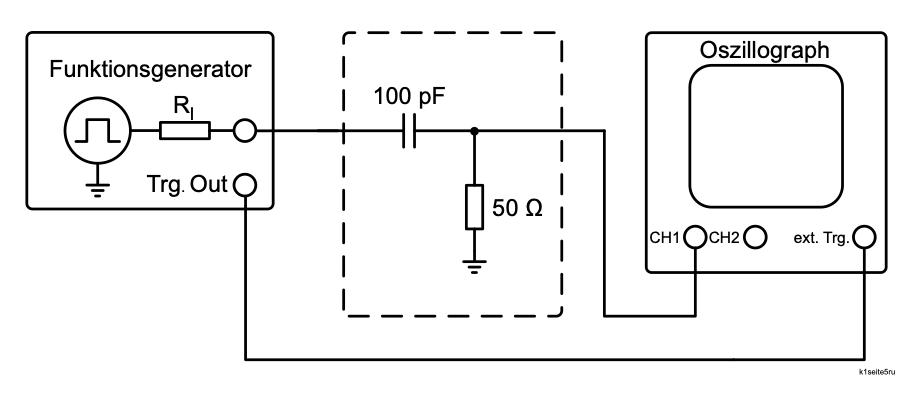
\includegraphics[width=0.8\textwidth]{Aufbau_1_1_Differenzierglied.png}
				\caption{Aufbau des Differenzierglieds~\cite{anleitung}}
				\label{fig:aufbau_1_1_differenzierglied}
			\end{figure}
			Ein RC-Glied wird (ohne $\SI{2.2}{\kilo\ohm}$ Abschluss) zwischen einen Funktionsgenerator und einen Oszillographen geschaltet. Der Funktionsgenerator wird auf eine Frequenz von $\SI{200}{\kilo\hertz}$ eingestellt. Dann wird das Oszillogramm gezeichnet und dasselbe mit dem $\SI{2.2}{\kilo\ohm}$ Abschlusswiderstand wiederholt.
			%TODO: Messwerte & Auswertung
		\end{aufgabe}
		\begin{aufgabe}{Impulse auf Kabeln}
			
			\begin{figure}[h!]
				\centering
				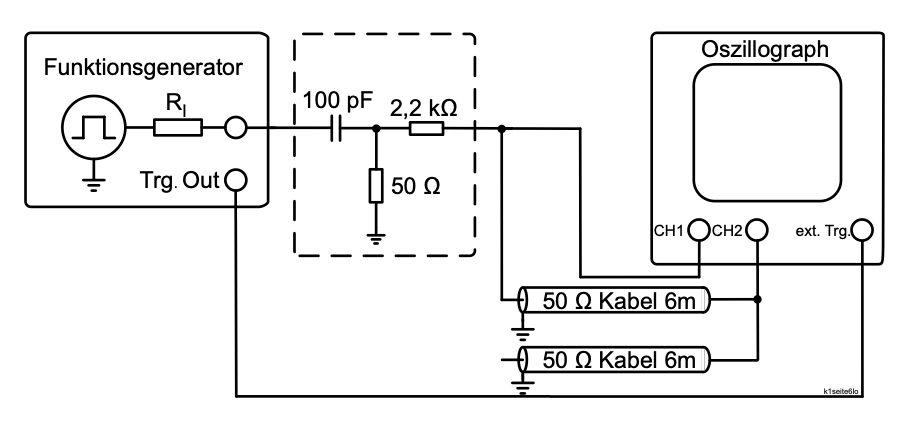
\includegraphics[width=0.8\textwidth]{Aufbau_1_2_Impulse_auf_Kabeln.png}
				\caption{Schaltplan für ein Kabel mit zwei offenen Enden~\cite{anleitung}}
				\label{fig:aufbau_1_1_impulseAufKabeln}
			\end{figure}
			Jetzt sollen die Impulse auf einem an beiden Enden offenen Kabel untersucht werden. Dazu wird ein Funktionsgenerator, welcher im Rechteckmodus mit $\SI{100}{\kilo\hertz}$ betrieben wird, vor ein RC-Glied mit Abschluss, welches als Impulsgeber dient, geschaltet. Diese Impulse werden einerseits im CH1 des Oszillographen angezeigt, andererseits durch zwei hintereinandergeschaltete Kabel mit jeweils $\SI{50}{\ohm}$ Wellenwiderstand geschickt. Zwischen den beiden Kabeln wird der Oszillograph im CH2 geschaltet. Der Funktionsgenerator dient als externer Trigger für den Oszillographen, die beiden Kanäle werden mit derselben Empfindlichkeit betrieben.

			
		\end{aufgabe}
		\begin{aufgabe}{Leitungsabschluss, Verzögerungszeit}
			\begin{figure}[h!]
				\centering
				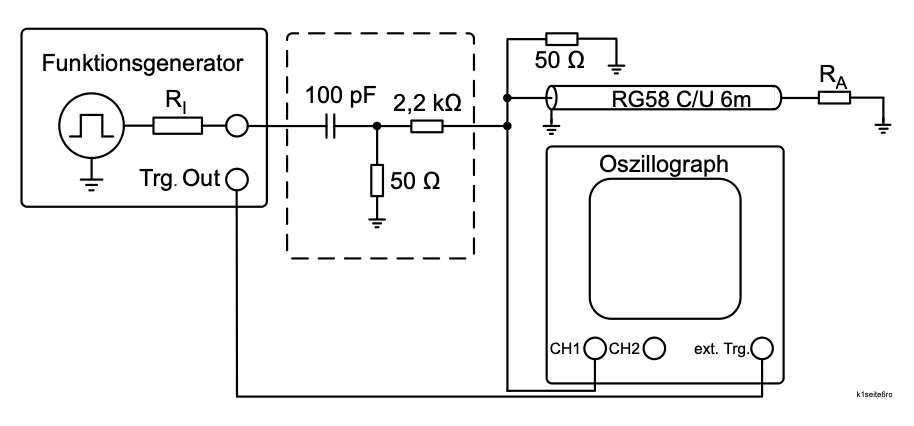
\includegraphics[width=0.8\textwidth]{Aufbau_1_3_Leitungsabschluss.png}
				\caption{Schaltplan für ein Kabel mit einem offenen und einem geschlossenen Ende~\cite{anleitung}}
				\label{fig:aufbau_1_3_leitungsabschluss}
			\end{figure}
			Nun wird die Auswirkung unterschiedlicher Leitungsabschlüsse auf die Impulse untersucht. Dazu wird weiterhin extern getriggert, der Impulsgenerator wird auch an CH1 angeschlossen. Statt der beiden Kabel wird jetzt mittels eines T-Stücks ein Verzögerungskabel mit $\SI{50}{\ohm}$ Wellenwiderstand und $\SI{6}{\meter}$ Länge verwendet, welches am anderen Ende mit einem Widerstand $R_\mathrm{A} = \SI{50}{\ohm}$ abgeschlossen ist. Es für jede der folgenden Anordnungen mit und ohne einem zusätzlichen Widerstand von $\SI{50}{\ohm}$ parallel zum Kabel gemessen:
			\begin{enumerate}[(a)]
				\item Offenes Ende
				\item Offenes Ende im Detail ($\times 10$)
				\item Kurzgeschlossenes Ende
				\item Kurzgeschlossenes Ende \& variierende Frequenzen (Zeitablenktung von $\SI{0.2}{\micro\second\per\centi\meter}$)
			\end{enumerate}
		\end{aufgabe}
		\begin{aufgabe}{Klippkabel, Dämpfung}
			\begin{figure}[h!]
				\centering
				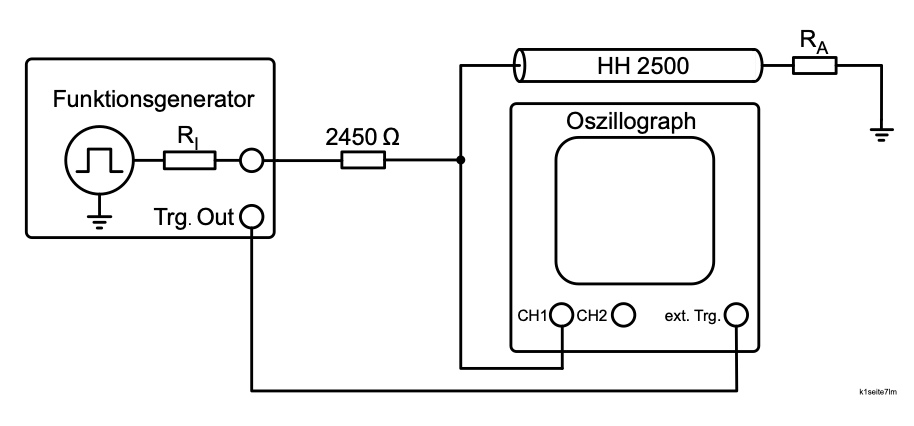
\includegraphics[width=0.8\textwidth]{Aufbau_1_4_Klippkabel.png}
				\caption{Schaltplan für ein Klippkabel~\cite{anleitung}}
				\label{fig:aufbau_1_4_klippkabel}
			\end{figure}
			Zuletzt wird das Verzögerungskabel mit einem kürzeren, sogenannten Klippkabel, mit $\SI{0.7}{\meter}$ Länge ersetzt. Anstatt des Differenzierglieds wird ein Widerstand von $\SI{2450}{\ohm}$ eingebaut, der Widerstand vor dem Kabel wird entfernt. Der Funktionsgenerator wird auf eine Frequenz zwischen $\SI{10}{\kilo\hertz}$ und $\SI{80}{\kilo\hertz}$ eingestellt. Die Schaltverbindungen erfolgen mit $\SI{50}{\ohm}$ Koaxialkabeln. Dann wird unter den folgenden Umständen am Oszillographen gemessen:
			\begin{enumerate}[(a)]
				\item Klippkabel mit $\SI{50}{\ohm}$ Abschluss, d.\ h.\ offen
				\item Klippkabel kurzgeschlossen
				\item Klippkabel kurzgeschlossen mit variierter Frequenz
				\item $\SI{2}{\meter}$ Klippkabel kurzgeschlossen 
			\end{enumerate}
		\end{aufgabe}
		
		%TODO Aufbau/Schaltskizze (beschrieben in wenigen Worten)
		%TODO Versuchsdurchführung: Messgrößen, unabh. Parameter, Messmethode, Einheiten, Genauigkeit, wie oft
		%TODO Abgezeichnetes Messprotokoll vorhanden?

		%TODO Auswertung (in Worten & Formeln)
		%TODO Formeln symbolisch und numerisch
		%TODO Runden
		%TODO Grafiken & Diagramme: Überschrift, Messwerte mit Fehlerbalken, (nur) gefittete Kurven, Achsenbeschriftung
		%TODO Fehlerrechnung und -diskussion
		%TODO Jede Tabelle eine Formel
	\section{Fazit}
		%TODO Vollständiger Satz fürs Endergebnis
		%TODO Messergebnisse bewerten und evtl. mit Literaturwerten vergleichen
		%TODO Untersuchung Fehlerquellen (statistisch, systematisch, blödsinnig)
	\printbibliography
\end{document}
